\section{Результаты работы}

Результатом работы является тестирование, разработанных программ на суперкомпьютере Polus. Для тестирования было выбрано количество процессоров равное 1, 2, 8, 20, 100 и входные данные N=\{200, 500, 700, 1000, 1200\}.
Из-за ограничения в 15 минут (900 секунд), для некоторых параметров значения так и не были получены. Эти параметры обозначены темно-синим цветом на диаграмме.


\begin{figure}[H]
    \centering
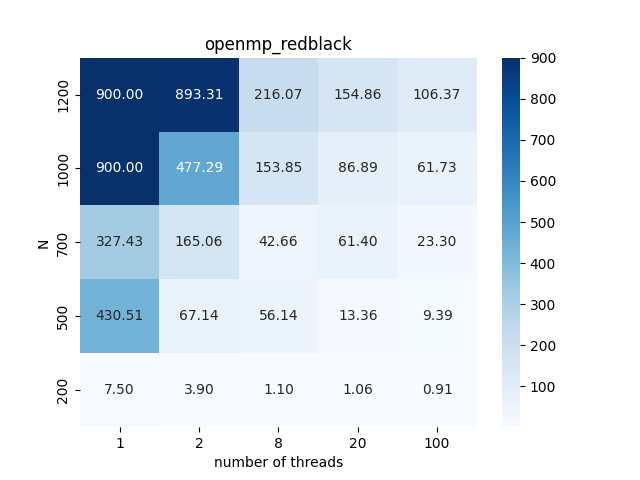
\includegraphics[width=1.\linewidth,center]{openmp_redblack.png}
    \caption{Алгоритм RedBlack3D}
\end{figure}

\begin{figure}[H]
    \centering
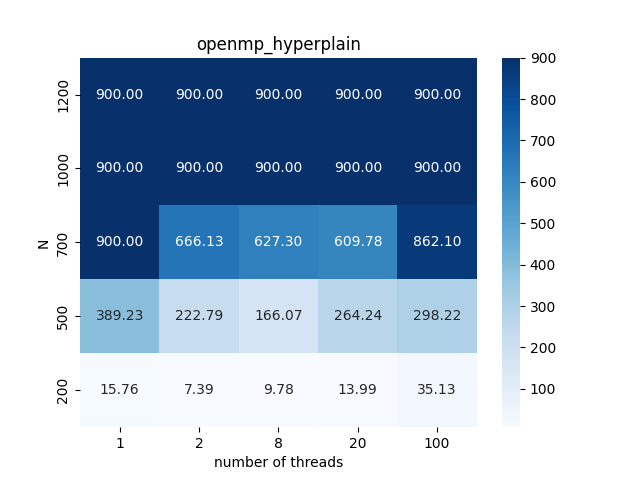
\includegraphics[width=1.\linewidth,center]{openmp_hyperplain.png}
    \caption{Распараллеливание по гиперплоскостям куба}
\end{figure}

Для визуализации данных была использована библиотека \code{seaborn} для \code{Python 3}.

